\documentclass[12pt,fleqn,twocolumn]{article}

\usepackage[english]{babel}
\usepackage[utf8]{inputenc}

\PassOptionsToPackage{hyphens}{url}\usepackage{hyperref}

\usepackage[top=2.5cm, bottom=2.5cm, left=3cm, right=3cm, includeheadfoot]{geometry}

\usepackage{fancyhdr}
\usepackage{graphicx}
\usepackage{float}
\usepackage{changepage}
\usepackage[nottoc, numbib]{tocbibind}
\usepackage{lastpage}
\usepackage{setspace}
\usepackage[bottom]{footmisc}
\usepackage{titling}

\usepackage{amsmath}
\usepackage{amssymb}
\usepackage{nicefrac}
\usepackage{icomma}

\usepackage{csquotes} % To avoid biber warnings
\usepackage[backend=biber, style=alphabetic, citestyle=alphabetic, maxcitenames=4, maxbibnames=4, mincitenames=2]{biblatex}
\usepackage{dirtytalk}

\mathcode`\*=\number\cdot
\newcommand{\numberthis}{\addtocounter{equation}{1}\tag{\theequation}}
\newcommand{\acomm}[1]{\hspace{2.5cm}\text{#1}}
\newcommand{\code}[1]{{\texttt{\small#1}}}

\newcommand{\md}{\ensuremath{\text{d}}}
\newcommand{\NN}{\ensuremath{\mathbb N}}
\newcommand{\ZZ}{\ensuremath{\mathbb Z}}
\newcommand{\QQ}{\ensuremath{\mathbb Q}}
\newcommand{\RR}{\ensuremath{\mathbb R}}
\newcommand{\CC}{\ensuremath{\mathbb C}}
\newcommand{\DD}{\ensuremath{\mathbb D}}
\newcommand{\LL}{\ensuremath{\mathbb L}}
\newcommand{\PP}{\ensuremath{\mathbb P}}
\newcommand{\transpose}[1]{\ensuremath{#1^{\textup T}}}

\newcommand{\half}{\ensuremath{\frac{1}{2}}}
\newcommand{\third}{\ensuremath{\frac{1}{3}}}
\newcommand{\fourth}{\ensuremath{\frac{1}{4}}}
\newcommand{\ctp}[1]{\ensuremath{\cdot10^{#1}}}
\newcommand{\reci}{\ensuremath{^{-1}}}

\usepackage[acronym, toc]{glossaries}
\newacronym{dl}{DL}{Deep Learning}
\newacronym{nlp}{NLP}{Natural Language Processing}
\newacronym{dp}{DP}{Differential Privacy}
\newacronym{ml}{ML}{Machine Learning}
\newacronym{dpsgd}{DP-SGD}{Differentially Private Stochastic Gradient Descent}
\newacronym{fl}{FL}{Federated Learning}
\newacronym{dpfa}{DP-FedAvg}{Differentially Private Federated Averaging}
\newacronym{adlm}{AdLM}{Adaptive Laplace Mechanism}



\addbibresource{references.bib}

\setlength{\droptitle}{-10ex}

\title{Hush-hush Gradients: A Review of Differential Privacy for Deep Learning}

\author{Søren Winkel Holm}
\date{\today}

\pagestyle{fancy}
\fancyhf{}
\lhead{Søren Winkel Holm}
\chead{}
\rhead{Technical University of Denmark}
\lfoot{Differential Privacy for Deep Learning}
\rfoot{Page \thepage{} of \pageref{LastPage}}

\graphicspath{{imgs/}}
\linespread{1.15}

\begin{document}
\setlength{\headheight}{15pt}
\addtolength{\topmargin}{-2.5pt}

\maketitle
\thispagestyle{fancy}
% \tableofcontents

\section*{Introduction}%
\label{sec:Introduction}
The field of \acrfull{dl} is for many subfields moving towards a setup where large multi-purpose foundation models are developed and trained at major companies or research instutitions, and then released for engineers to adapt to specific applications \cite[pp. 3]{bommasani2021oppurt}.
This application of the open-source principle to pre-trained models improves scientific reproduction ability \cite[pp. 3]{hartley2020dtool} and technology accessibility \cite[pp. 139]{bommasani2021oppurt}.
One risk, however, is an adversarial actor exploiting a property of \acrshort{dl} models: 
Parts of training data is generally recoverable from model weights \cite{nasr2019privacy, shokri2017membership}.
This might expose proprietary data or the private data of individuals as exemplified for \acrfull{nlp} language models in Figure \ref{fig:extracting.pdf}.
As large-scale data sets are here to stay \cite{sun2017unreasonable}, algorithmic methods for improving the privacy of foundation models are required.
The methods of \acrfull{dp} are suitable for this task and the relevant concepts, algorithms and problems will here be reviewed.

\begin{figure}[H]
    \centering
        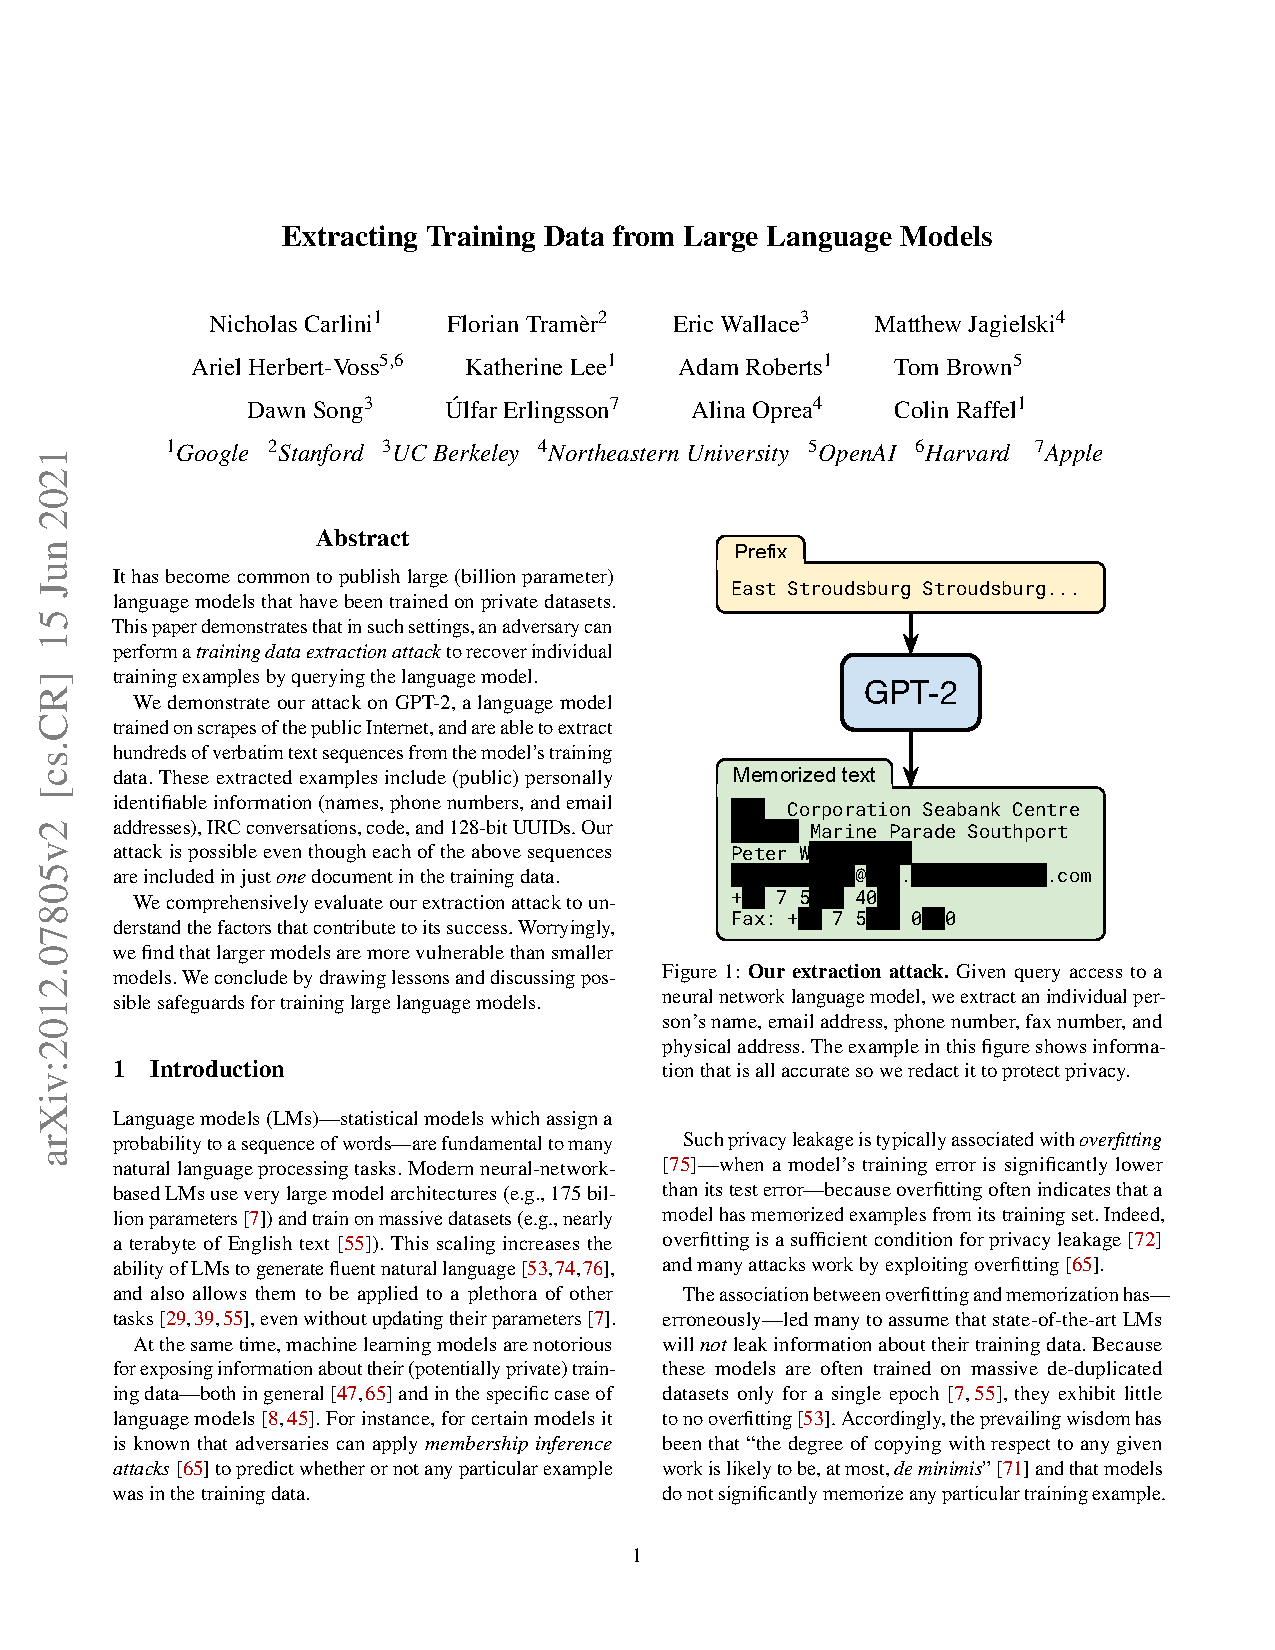
\includegraphics[clip, trim=11.5cm 12cm 2.5cm 8cm, width=.8\linewidth]{extracting.pdf}
        \caption{The extraction attack performed on GPT-2 \cite[Fig. 1]{carlini2021extracting} (private data redacted).}
    \label{fig:extracting.pdf}
\end{figure}\noindent

\section*{Fundamental Concepts}%
\label{sec:Fundamental Concepts}
Achieving \acrshort{dp} corresponds to making a promise of hiding information about individuals when publishing quantitative patterns about groups \cite[pp. 5]{dwork2014alg}.
This general problem is historically faced in releases of statistical data analyses by e.g. official organizations \cite{dalenius1977stat, wiki2022diff}.
An algorithm is thus differentially private if a third party observer cannot extract individual information from its' computation.
In this context, a \acrfull{ml} model \(f(x|w)=\hat y \approx y\) trained on a data set \(\mathcal D\) exposes data patterns when either its' parametrization $w$ or predictions $(x, \hat y)$ are released.

Let $\mathcal D_i \in \DD$ be a data set containing the private information of individual $i$ and $\mathcal D_{\hat i} \in \DD$ be identical except excluding this private information.
For most approaches, the goal is to maximise \acrshort{dp} by minimising the impact of individual data on computation which can be be quantified by measures such as $\ell_1$-sensitivity \cite[pp.31]{dwork2014alg} $\Delta g$ of a numeric statistic $g: \DD \rightarrow \RR^k$,
\begin{equation}
    \Delta g= \operatorname{max}_{i, \hat i \in \DD} ||g(x)-g(y)||_1.
\end{equation}
To achieve this, additive noise mechanisms can be used.
For $\Delta g$, this can be achieved by adding Gaussian noise to outputs \cite[D 3.3]{dwork2014alg} 
\begin{equation}\label{eq:gauss}
  f(x)+(Y_1, \ldots, Y_k), Y_i \sim \mathcal N(0, \sigma_{\Delta g}^2)  
\end{equation}
The end goal of such \acrshort{dp} mechanisms on random algorithms $\mathcal F(\mathcal D)$ outputting $w \in \operatorname{Im}(\mathcal F)$ with probability $p_{\mathcal F}(w|\mathcal D)$, is to guarantee $(\varepsilon, \delta)$-privacy \cite[Def. 2.4]{dwork2014alg} requiring $\forall S \in \operatorname{Im}(\mathcal F)$ that
\begin{equation}
    P\left(
        \mathcal{F}(\mathcal D_i) \in S
    \right)
    \leq
    \exp(\varepsilon)
    P\left(
        \mathcal{F}(\mathcal D_{\hat i}) \in S
    \right)
    +\delta.
\end{equation}
Thus, for $1-\delta$ of the probability density over algorithmic randomness, it is promised that adding your private data to $\mathcal D$ does not raise your risk of harm by more than $\exp(\varepsilon)$ \cite[pp. 21]{dwork2014alg}.
Often, $\delta=0$, requring the stronger $\varepsilon$-privacy \cite{wiki2022diff}.
For the Gaussian additive noise mechanism \eqref{eq:gauss}, $(\varepsilon, \delta)$-privacy is achieved when $\sigma_{\Delta g}^2=\Delta g \ln(\nicefrac 1 \delta)\varepsilon\reci$ \cite[App. A]{dwork2014alg}.

\section*{State of the Art}%
\label{sec:State of The Art}

\section*{Open Problems}%
\label{sec:Open Problems}

\clearpage
\renewcommand*{\bibfont}{\normalfont\footnotesize}
\printbibliography[heading=bibintoc]

\printglossary[type=\acronymtype]

\end{document}
